\documentclass[border=5pt]{standalone}
\usepackage{tikz}
\usetikzlibrary{arrows.meta, 3d, perspective, calc}
\usepackage{amsmath}
\begin{document}
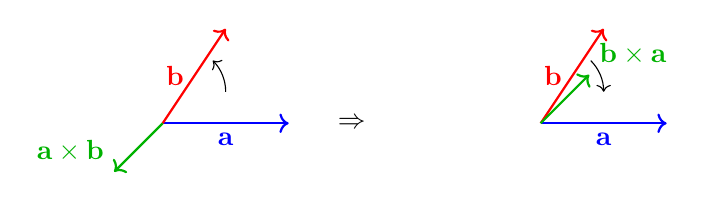
\begin{tikzpicture}[scale=0.8]
    % First diagram: a × b
    \begin{scope}[shift={(-3,0)}]
        \draw[->,thick,blue] (0,0) -- (2,0) node[midway,below] {$\mathbf{a}$};
        \draw[->,thick,red] (0,0) -- (1,1.5) node[midway,left] {$\mathbf{b}$};
        \draw[->,thick,green!70!black] (0,0) -- (0,0,2) node[above left] {$\mathbf{a} \times \mathbf{b}$};
        \draw[->] (1,0.5) arc (0:45:0.7);
    \end{scope}

    % Second diagram: b × a
    \begin{scope}[shift={(3,0)}]
        \draw[->,thick,red] (0,0) -- (1,1.5) node[midway,left] {$\mathbf{b}$};
        \draw[->,thick,blue] (0,0) -- (2,0) node[midway,below] {$\mathbf{a}$};
        \draw[->,thick,green!70!black] (0,0) -- (0,0,-2) node[above right] {$\mathbf{b} \times \mathbf{a}$};
        \draw[<-] (1,0.5) arc (0:45:0.7);
    \end{scope}

    % Middle text
    \node at (0,0) {$\Rightarrow$};
\end{tikzpicture}
\end{document}
